\documentclass{article}
\usepackage[utf8]{inputenc}
\usepackage{graphicx}
\usepackage{float}
\graphicspath{ {./images/} }
\usepackage{amssymb}

\title{IsLeapYear}
\author{Patrick Bohn Matthiesen}
\date{}

\begin{document}

\maketitle
My take on the algorithm is just to check if the year modulo 4 is equal to 0, and then to make sure a year like 200 do not work for the rule, that it can not be divisible by 100. To support the third rule that anything divisible by 400 is a leap year, an "or" is placed as a secondary condition.
\begin{figure}[h]
\centering
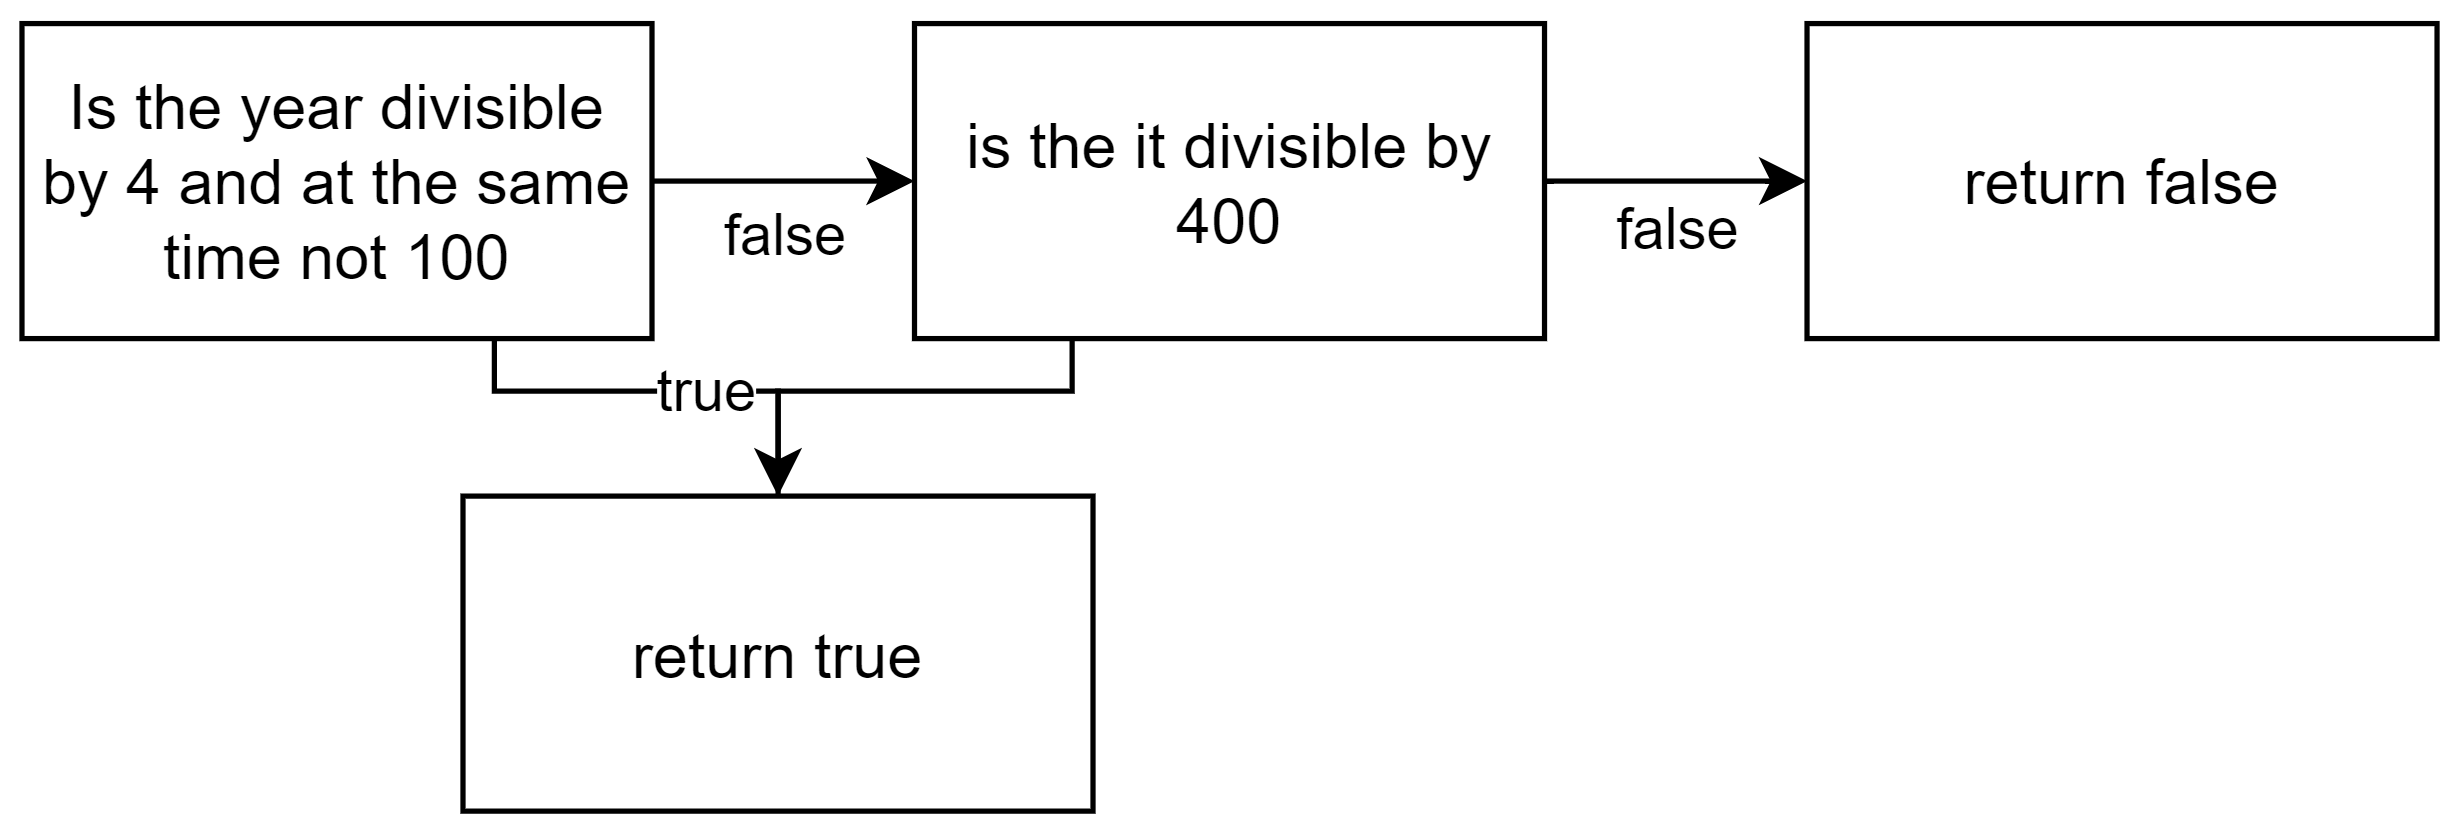
\includegraphics[width=\textwidth]{images/image.png}
\end{figure}


\end{document}
